\documentclass{article}

\usepackage{graphicx} % Required for the inclusion of images
\usepackage{natbib} % Required to change bibliography style to APA
\usepackage{amsmath} % Required for some math elements 
\usepackage{url}
\usepackage{hyperref}
\usepackage{listings}
\usepackage{textcomp}
\setlength\parindent{0pt} % Removes all indentation from paragraphs

\usepackage{geometry}
 \geometry{
 total={210mm,297mm},
 left=20mm,
 right=20mm,
 top=40mm,
 bottom=20mm,
 }

\title{RNA-Seq Analysis Report}
\author{Center For Cancer Computational Biology \\ Dana Farber Cancer Institute}

\begin{document}

\maketitle

\section{Introduction}
This report summarizes the processes used in analyzing your data. For further questions regarding details of the analysis, please contact the CCCB.

\section{Alignment}
Alignments were performed with STAR aligner  (version 2.5) \cite{star} which is specifically designed for RNA-Seq experiments, which may include multiple splice forms and fusion transcripts.  Not all aligners produce the same results, as sequencing mistake, low--complexity sequences, variants, and other factors are treated differently and may affect the quality of the resulting alignment to the reference genome.\\

The output from the alignment is in a compressed, binary format-- a BAM file.  You cannot open and read BAM files as you might a regular text file.  Although not often necessary, text representations of the BAM file (SAM format) may be generated with software such as samtools \cite{samtools}.\\

Following the alignment, the BAM files are passed through several processing steps.  For our standard processes, we create three levels of BAM file:
\begin{itemize}
\item *.sort.bam \\
These BAM files are sorted by genomic coordinates, which is necessary for tools such as IGV (see Section \ref{sec:igv})
\item *.sort.primary.bam \\
To obtain these BAM files we filter the sorted BAM files to retain only ``primary'' alignments.  When sequencing reads are aligned to the reference genome, it is possible that they may align well to multiple locations due to homology, paralogous genes, low-complexity regions, sequencing errors, or any number of other factors.  The aligner scores the quality of the alignment and marks some reads as secondary.  Thus, the primary-filtered files retain only the most high-quality reads for downstream analysis.  We recommend using these BAM files for further downstream analysis.  
\item *.sort.primary.dedup.bam \\
These are BAM files which remove reads that are marked as duplicates.  Here, duplicates are defined as reads that align to the same exact genomic coordinates and have the same sequence.  In whole-genome DNA sequencing, the random fragmentation results in a very low probability of two identical pieces of DNA; reads that are exact copies are most likely artifacts of PCR amplification and should be discarded.  While PCR-based duplication is still a problem for low-quantity RNA-Seq experiments there is increasing evidence that the removal of duplicate reads unnecessarily discards good data, perhaps affecting the eventual testing for differential expression.  Since only a small portion of the genome is sampled in a RNA-Seq experiment, it is more likely that the fragmentation of distinct transcripts can result in identical RNA fragments.  Illumina has reported on internal studies which used unique sequence barcodes to distinguish PCR-based duplicates from duplicate reads originating from distinct transcripts.  Their data suggest that it is good practice to retain the duplicate reads.  However, it is important to appreciate that there is still some debate surrounding this matter.  
\end{itemize}

In our convention, the asterisk (*) is the sample identifier and there are three BAM files for each sample.  To reduce the number of files for download, however, we only offer the *.sort.primary.bam as it
is usually the most appropriate file to use for differential expression analysis.  If there is a high level of duplication, it might be better to use the deduplicated BAM files.  These can be made available by request to the CCCB.

Brief alignment metrics are shown below in Figures \ref{fig:relative_composition} and \ref{fig:total_counts}:

\begin{figure}[ht!]
  \centering
    \includegraphics[width=0.75\textwidth]{mapping_composition}
    \caption{The relative composition of reads from alignment.}
    \label{fig:relative_composition}
\end{figure}

\begin{figure}[ht!]
  \centering
    \includegraphics[width=0.75\textwidth]{total_reads}
    \caption{The total reads from the experiment.}
     \label{fig:total_counts}
\end{figure}



\section{Read quantification}

For this analysis, reads and differential expression analysis are treated at the gene level, as opposed to inference about specific transcript abundance.  Even at the simpler level of counting reads at the gene level, there are subtle issues in just how you perform this.
For this task we use featureCounts software \cite{featureCounts} which produces integer counts for all genes in the supplied genome annotation file (GTF format).  We note that sequencing reads are counted to the annotated coding regions (CDS).\\

The resulting counts are arranged into an expression matrix such as,
\begin{center}
\begin{tabular}{c || c | c | c | r }
  Gene & SampleA & SampleB & SampleC & \ldots \\
  \hline			
  X & 1 & 2 & 3 & \ldots \\
  Y & 4 & 5 & 6 & \ldots\\
  Z & 7 & 8 & 9 & \ldots\\
  \hline  
\end{tabular}
\end{center}

Files containing the information are termed the ``raw'' counts and are available at all three filter levels described for the BAM files.  However, for the reasons outlined above, we only make the ``primary filtered'' available by default.  These are tab-delimited files and may be opened with a spreadsheet program such as Excel; however, we caution that Excel can lead to unexpected errors in the gene names \cite{excel}.


\section{Differential expression analysis (if performed)}

For differential gene expression analysis, we use DESeq2 \cite{deseq2} software, part of R's Bioconductor software library.  In brief, this software works by estimating the mean and variance of each gene's expression based on the 
alignment counts.  Using an assumed negative-binomial model for the counts, a statistical test is performed to assess differential expression.  This provides the p-value, given in the \verb|pvalue| column.  

Given the large number of statistical tests performed (basically one for each gene with some caveats), it is important to use "multiple-test corrections" to limit false-positives when judging differential expression.
This information is found in the \verb|padj| column.  A common threshold value for judging differential expression is $padj < 0.05$, although this threshold is effectively arbitrary, aimed at keeping the number of false positive genes to at most 5\%.  If there are relatively few genes passing this threshold, one may sort by the \verb|pvalue| column to assess potentially differentially expressed transcripts.\\

Our best advice is to use the list as a guide to inform additional analyses such as those interrogating biological pathways/processes.  

\section{Viewing your alignment data}
\label{sec:igv}
For viewing the BAM files, we recommend downloading and installing the Integrated Genomics Viewer (IGV), released by the Broad Institute.  This software runs on platforms with a Java installation (Windows, Mac, Linux/Unix) and can help to view more informationa about your experiment, including detection of problems. \\

In Figure \ref{fig:igv_dups}, we have focused on a $~1800$bp region in an exon of the MALAT1 gene where one can see very non-uniform read distribution across this particular exon.  One location in particular has many sequencing reads stacked on top of one another, with very minimal random tiling/overlap.  In addition, the red color indicates that all the reads originated from a single strand.  A more typical alignment shown in Figure \ref{fig:igv_typical} shows a mix of plus and minus-strand reads and random tiling/overlap.

\begin{figure}[ht!]
  \centering
    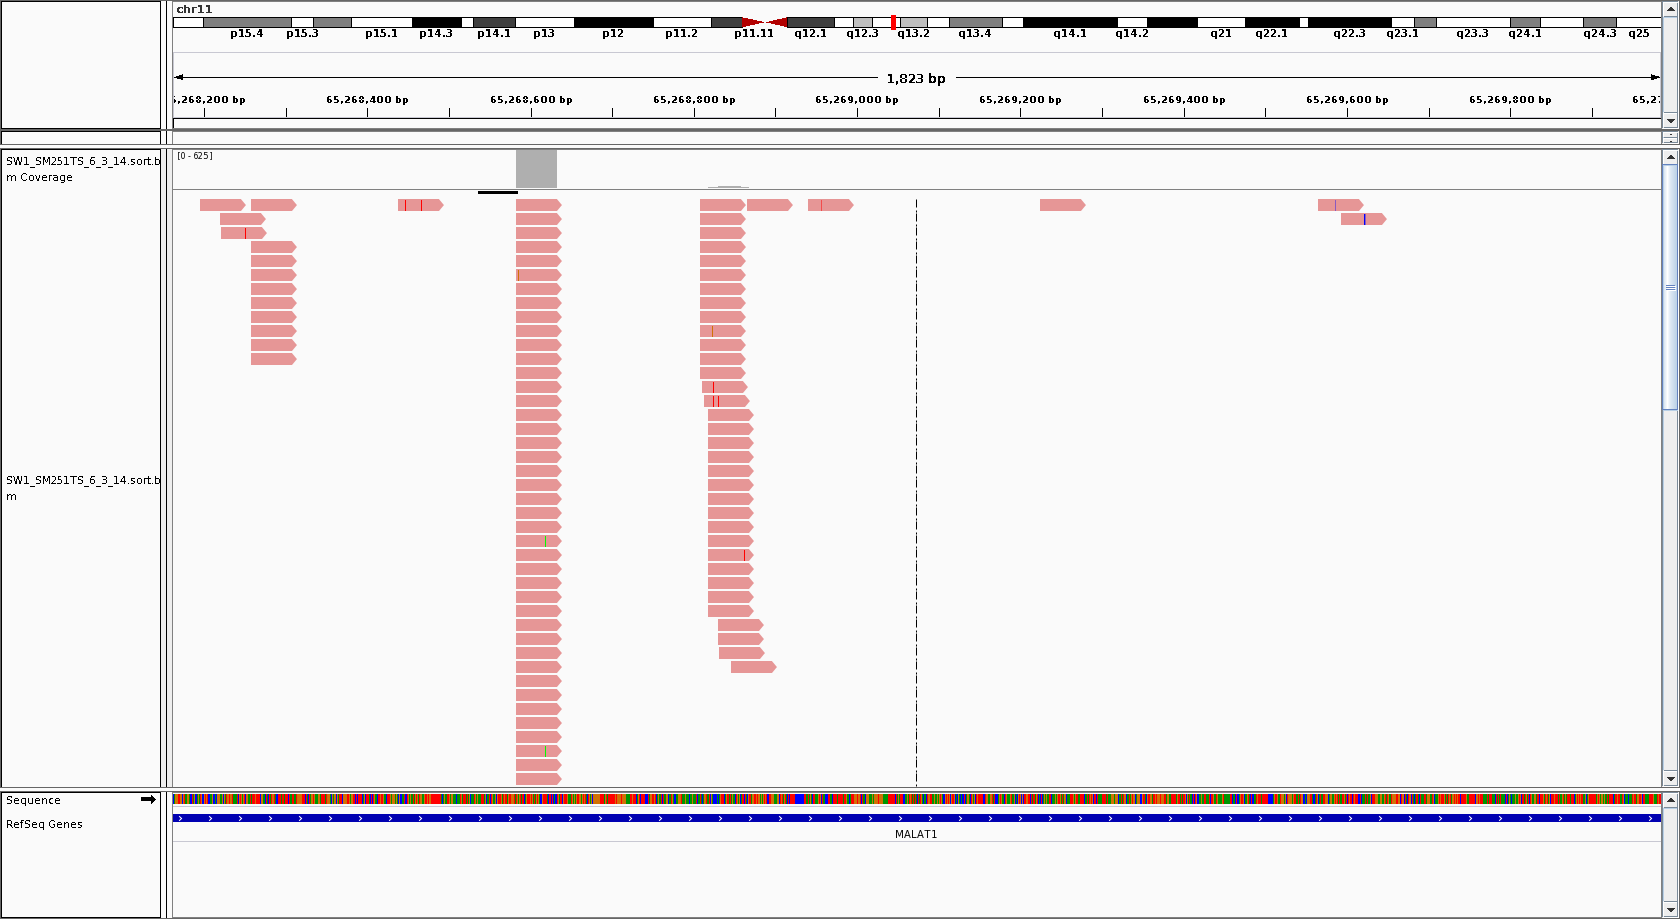
\includegraphics[width=0.75\textwidth]{igv_duplicates.png}
    \caption{IGV screenshot.  Many duplicate reads are visible.}
     \label{fig:igv_dups}
\end{figure}

\begin{figure}[ht!]
  \centering
    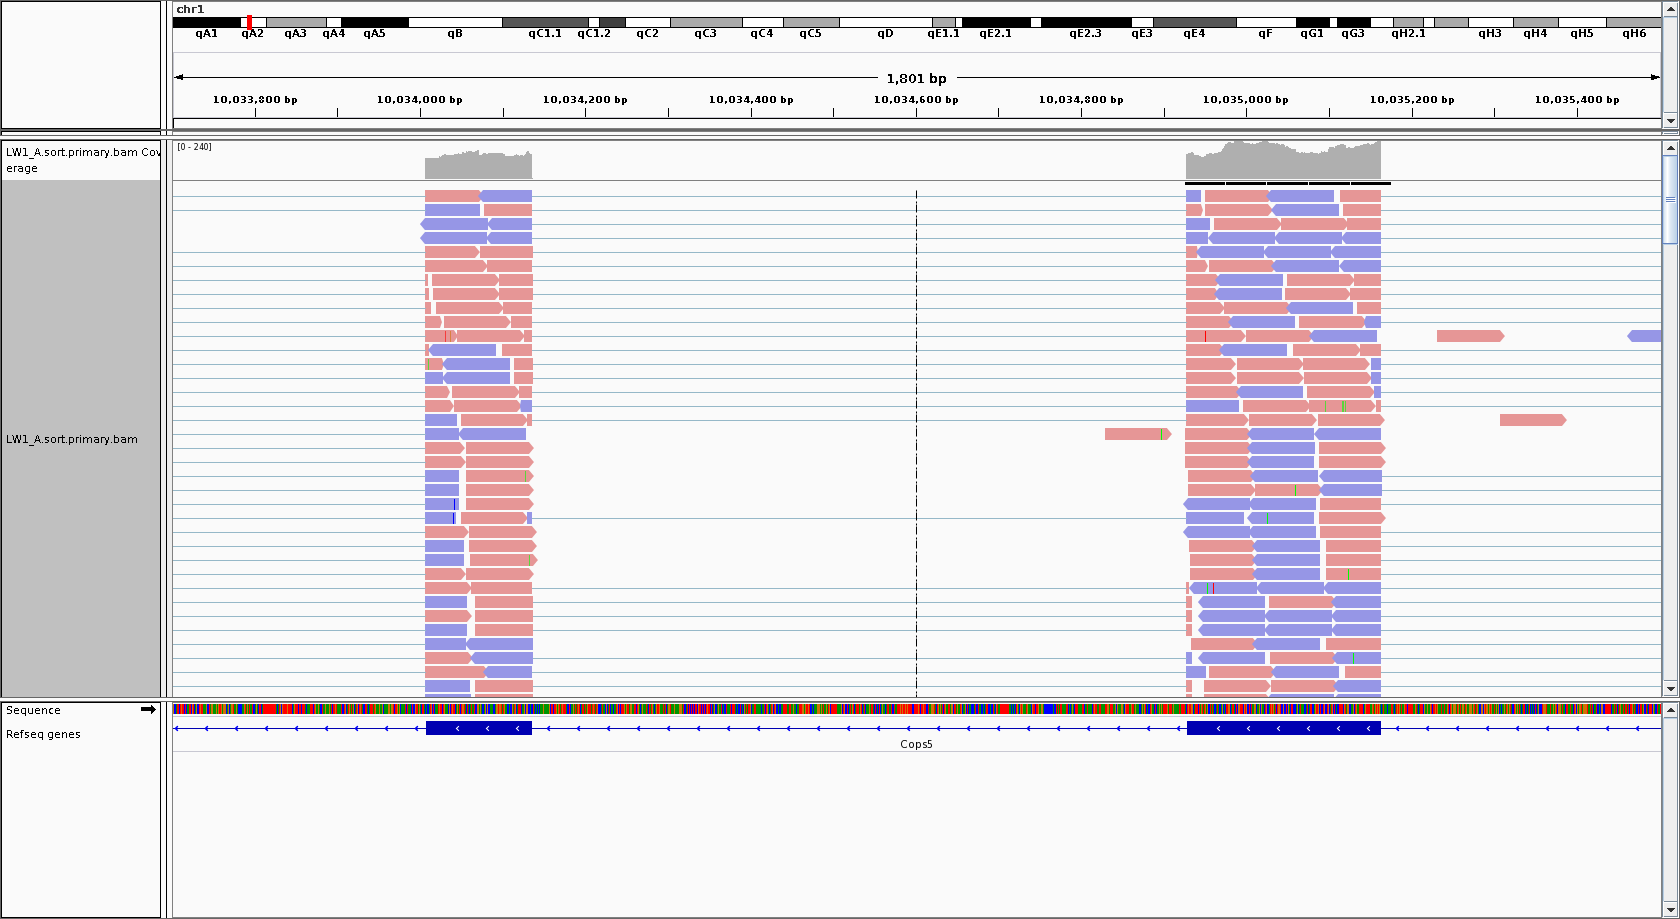
\includegraphics[width=0.75\textwidth]{igv_typical.png}
    \caption{IGV screenshot.  A more ``typical'' picture of read alignments.}
     \label{fig:igv_typical}
\end{figure}

\bibliographystyle{plain}

\bibliography{references}


\end{document}

